\documentclass[xcolor=table]{beamer}

\usepackage{lscape, amsmath, amsfonts, amssymb, setspace, theorem, wrapfig, graphicx, float, multirow, subfig, color, rotating, multicol, datetime, natbib, venndiagram, pstricks, xkeyval, tikz, etoolbox, verbatim, subfig}

\usepackage[super]{nth}
\usepackage{listings}
\usepackage{xcolor}

\definecolor{codegreen}{rgb}{0,0.6,0}
\definecolor{codegreengray}{rgb}{0,0.4,0}
\definecolor{codegray}{rgb}{0.5,0.5,0.5}
\definecolor{codeblue}{rgb}{0.00,0,0.82}
\definecolor{backcolour}{rgb}{0.95,0.95,0.92}
 
\lstdefinestyle{mystyle}{
    backgroundcolor=\color{backcolour},   
    commentstyle=\color{codegreengray},
    numberstyle=\tiny\color{codegray},
    stringstyle=\color{codegreen},    basicstyle=\ttfamily\footnotesize,
    breakatwhitespace=false,         
    breaklines=true,                 
    captionpos=b,                    
    keepspaces=true,                 
    numbers=left,                    
    numbersep=5pt,                  
    showspaces=false,                
    showstringspaces=false,
    showtabs=false,                  
    tabsize=2
}
 
\lstset{style=mystyle}

\title{GV300 - Quantitative Political Analysis}
\subtitle{University of Essex - Department of Government}
\date{Week 11 -- 9 December, 2019}				% or you can specify a date, just write it down instead of "\today"
\author{Lorenzo Crippa} 

\usetheme[progressbar=frametitle]{metropolis}
\usecolortheme{seahorse}						% try others: wolverine; crane...


\begin{document}

\frame{
\titlepage
}

\frame{
\frametitle{Problem Set 4.1}
\begin{enumerate}
\item (15 marks) Reviewing regression analysis basics: normal, t, $\chi^2$ and F distributions. You will use your preferred statistical software for this exercise. 
\end{enumerate}
}

\frame{
\frametitle{Problem Set 4.1}
\begin{enumerate}
\item[(a)] (3 marks) generate a dataset with 2000 observations and create three variables each with values drawn from a standard normal distribution. \pause
For each variable \textbf{show that roughly 68\% of the observations are within 1 standard deviation of 0, 95\% within two standard deviations of 0, and 99\% are within 3 standard deviations of zero.}
\end{enumerate} \pause

Show that roughly 68\% of \textbf{your} observations are within 1 standard deviation of the mean, 95\% within two standard deviations of the mean, and 99\% are within 3 standard deviations.
}

\frame{
\frametitle{Problem Set 4.1}
(a) First determine (or represent) your three intervals. \pause With a plot:
\begin{figure}
\centering
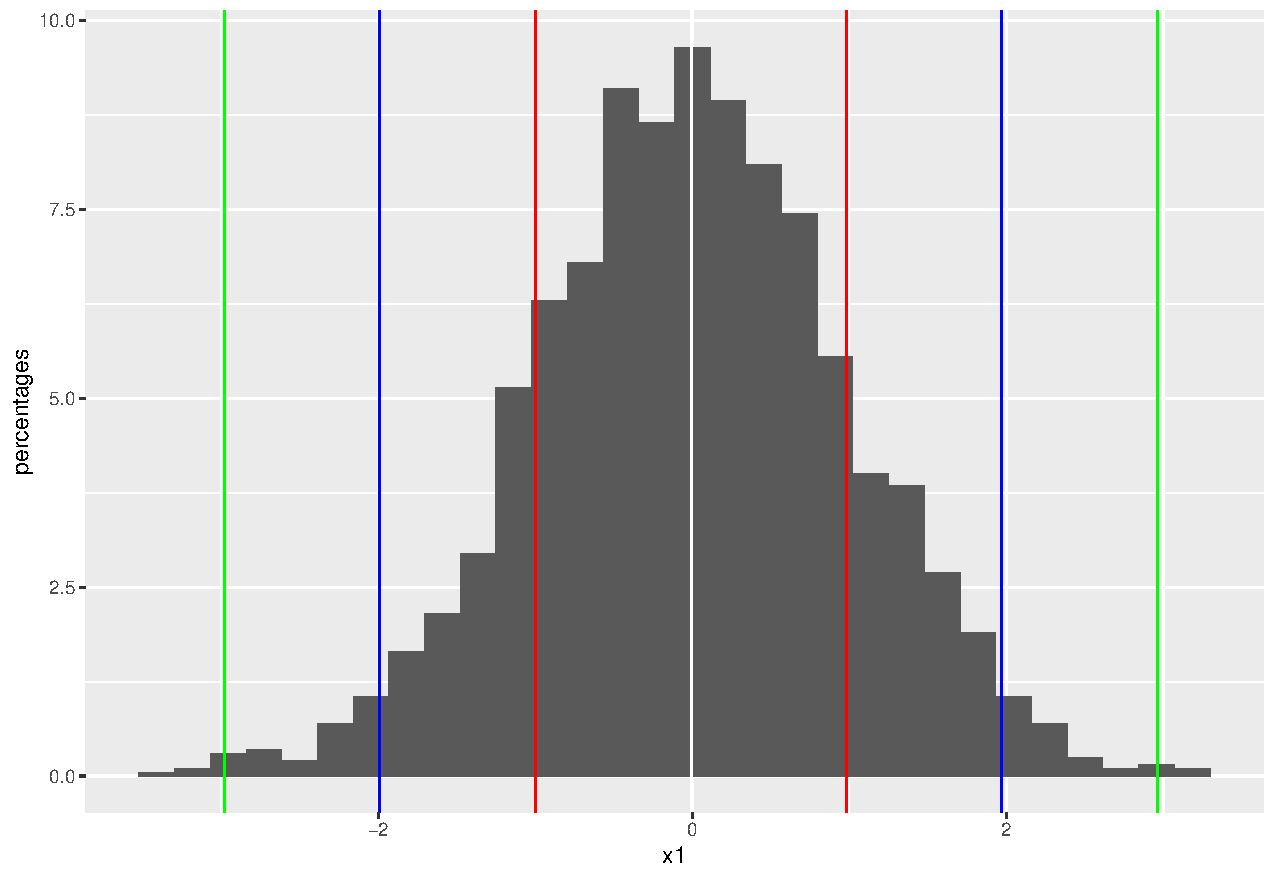
\includegraphics[width=100mm]{pictures/problemset4_hist.pdf}
\end{figure}
}

\begin{frame}[fragile]
\frametitle{Problem Set 4.1}
(a) Then use a percentile function. \pause In R: \pause
\begin{lstlisting}[language = R]
quantile(df$x1, probs = c(.005, .025, .16, .84, .975, .99))
\end{lstlisting} \pause

In Stata: 
\begin{lstlisting}
centile x1, centile(.5 2.5 16 84 97.5 99)
\end{lstlisting} \pause

Output:
\begin{lstlisting}[language = R]
      0.5%       2.5%        16%        84%
-2.7398407 -1.9486126 -0.9676747  0.9748144

      97.5%        99% 
  1.8915366  2.2497764 
\end{lstlisting} \pause

Repeat the same procedure for all variables
\end{frame}

\frame{
\frametitle{Problem Set 4.1}
\begin{enumerate}
\item[(b)] (3 marks) \textbf{Show that 95\% of the observations of a $\chi^2[1]$-distributed variable that you create are below the value that is associated with the \nth{95} percentile of the $\chi^2[1]$-distribution.} \pause If you are unsure about how to do this, plot the $\chi^2[1]$-distribution and eye-ball which value is associated with the $.95$-percentile of that distribution.
\end{enumerate}
}

\frame{
\frametitle{Problem Set 4.1}
(b) Distribution of a $\chi^2[1]$-distributed variable:
\begin{figure}
\centering
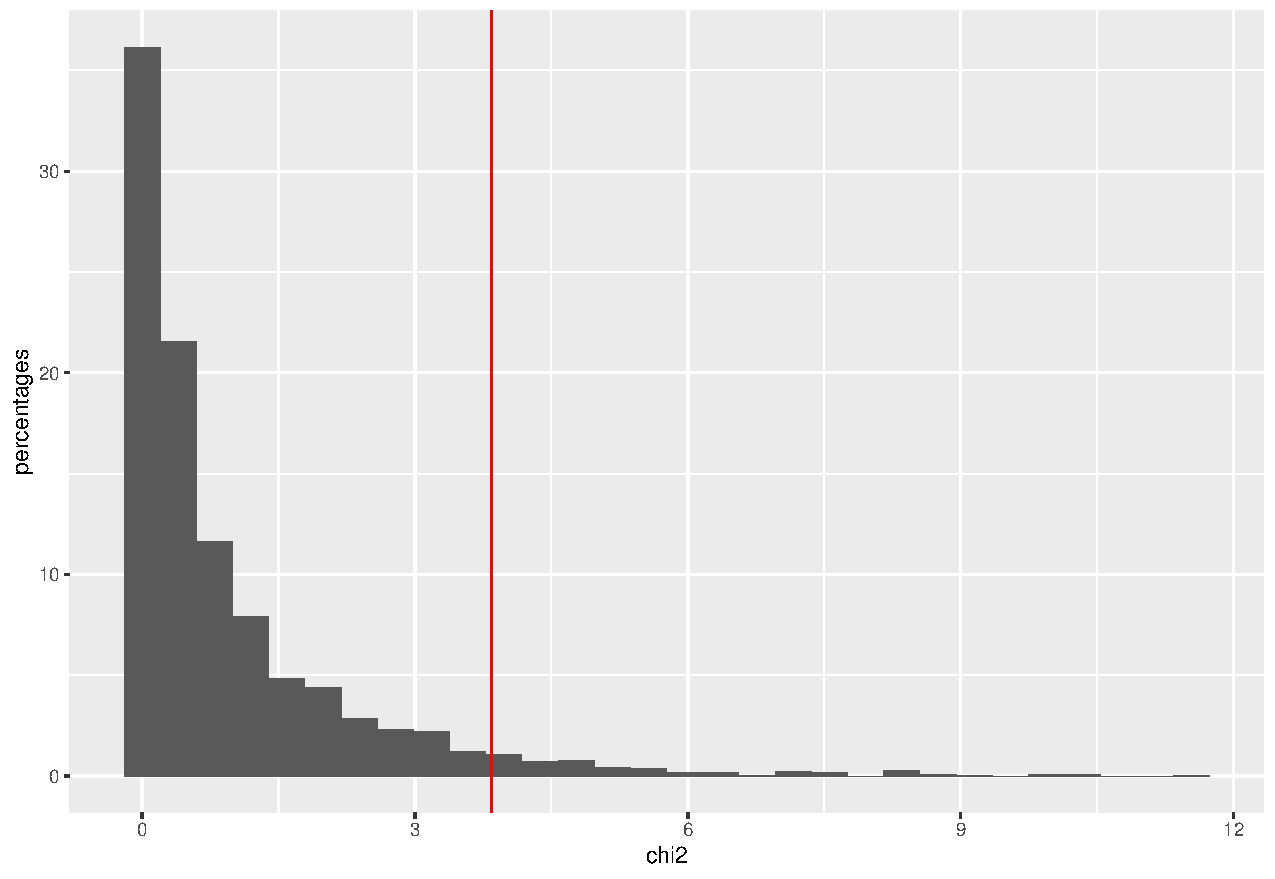
\includegraphics[width=100mm]{pictures/problemset4_hist_chi2.pdf}
\end{figure}
}

\begin{frame}[fragile]
\frametitle{Problem Set 4.1}
(b) From tables we know that \nth{95} percentile of a $\chi^2[1]$ distribution is $3.84$ \pause Again, we use a percentile function. \pause

In R: \pause
\begin{lstlisting}[language = R]
quantile(df$chi2, probs = .95)
\end{lstlisting} \pause

In Stata: 
\begin{lstlisting}
centile chi2, centile(95)
\end{lstlisting} \pause

Output:
\begin{lstlisting}[language = R]
     95% 
3.764813 
\end{lstlisting}
\end{frame}

\frame{
\frametitle{Problem Set 4.1}
\begin{enumerate}
\item[(c)] (3 marks) \textbf{Now, show that 95\% of the observations of a $F[1,1]$ distributed variable that you create are below the value that is associated with the $.95$-percentile of the $F[1,1]$-distribution.}
\end{enumerate}
}

\frame{
\frametitle{Problem Set 4.1}
(c) Distribution of an $F[1,1]$-distributed variable:
\begin{figure}
\centering
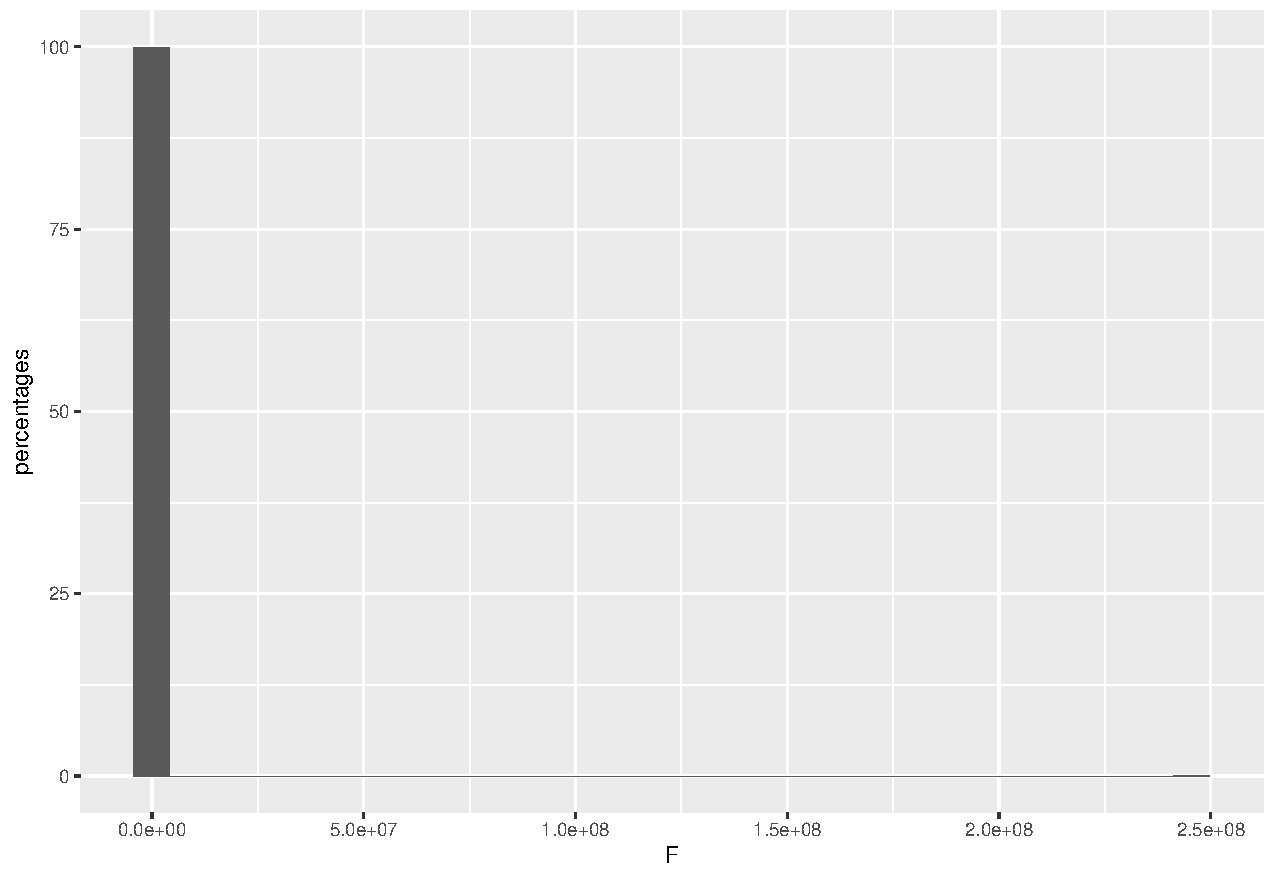
\includegraphics[width=100mm]{pictures/problemset4_hist_F.pdf}
\end{figure}
}

\begin{frame}[fragile]
\frametitle{Problem Set 4.1}
(c) From tables we know that \nth{95} percentile of a $F[1,1]$ distribution is $161.4$ \pause Again, we use a percentile function. \pause

In R: \pause
\begin{lstlisting}[language = R]
quantile(df$F, probs = .95)
\end{lstlisting} \pause

In Stata: 
\begin{lstlisting}
centile F, centile(95)
\end{lstlisting} \pause

Output:
\begin{lstlisting}[language = R]
     95% 
168.6171 
\end{lstlisting}
\end{frame}

\frame{
\frametitle{Problem Set 4.1}
\begin{enumerate}
\item[(d)] (3 marks) Take one of the variables with a standard normal distribution from (a) and divide it by the square root of the $\chi^2[1]$-distributed variable you created in (b). \pause Show that 95\% of the observations of that new variable are below the value that is associated with the $.95$-percentile of the t-distribution. \pause For what purpose do we usually compute a t-statistic in regression analysis and how is it computed? \pause How does the computation of the t-statistic in regression analysis link to how you computed the new variable here in exercise (d)?
\end{enumerate}
}

\frame{
\frametitle{Problem Set 4.1}
(d) Distribution of a $t[1]$-distributed variable:
\begin{figure}
\centering
\includegraphics[width=100mm]{pictures/problemset4_hist_t.pdf}
\end{figure}
}

\begin{frame}[fragile]
\frametitle{Problem Set 4.1}
(d) From tables we know that \nth{95} percentile of a $t[1]$ distribution is $6.314$ \pause Again, we use a percentile function. \pause

In R: \pause
\begin{lstlisting}[language = R]
quantile(df$t, probs = .95)
\end{lstlisting} \pause

In Stata: 
\begin{lstlisting}
centile t, centile(95)
\end{lstlisting} \pause

Output:
\begin{lstlisting}[language = R]
     95% 
7.136391 
\end{lstlisting}
\end{frame}

\frame{
\frametitle{Problem Set 4.1}
\begin{enumerate}
\item[(d)] (3 marks) For what purpose do we usually compute a t-statistic in regression analysis and how is it computed? \pause How does the computation of the t-statistic in regression analysis link to how you computed the new variable here?
\end{enumerate}

We compute the t-statistic to conduct a hypothesis test about the size of the coefficient estimate. \pause 

The t-statistic is computed from the ratio of coefficient estimate minus reference value (most often zero, regression outputs report a zero reference value by default) and standard error of the estimate. \pause

The t-statistic is the ratio between OLS estimates (which have a standard normal distribution) and standard errors (squared roots of the variance, which has a $\chi^2$ distribution)
}

\begin{frame}
\frametitle{Problem Set 4.1}
\begin{enumerate}
\item[(e)] (3 marks) Plot all variables you created so far, that is, three variables with a standard normal distribution, one variable distributed $\chi^2[1]$, one variable distributed $F[1,1]$, and one variable following the t-distribution. 
\end{enumerate} \pause

See previous graphs (histograms, but also densities \ldots)
\end{frame}

\frame{
\frametitle{Problem Set 4.2}
\begin{enumerate}
\item[2.] (24 marks) Linking conditional expectation function and linear regression function. Load the dataset \texttt{baseball.csv}. It gives you information on a series of MLB players on their height in inches (variable \emph{heightinches}) and weight (\textit{weightpounds}).
\end{enumerate}
}

\begin{frame}[fragile]
\frametitle{Problem Set 4.2}
(a) Generate the expected value of height for each value of weight. \pause It is simply the mean for values of weight (89 cases). \pause In R: \pause
\begin{lstlisting}[language = R]
aggregate(data$heightinches, by = list(data$weightpounds), FUN = mean)
\end{lstlisting} \pause

In Stata: 
\begin{lstlisting}
tabstat heightinches, by(weightpounds)
\end{lstlisting} \pause

Output:
\begin{lstlisting}[language = R]
   Group.1        x
1      150 70.75000
2      155 69.33333
3      156 75.00000
4      160 71.46667
5      163 70.00000
...    ...
\end{lstlisting}
\end{frame}

\frame{
\frametitle{Problem Set 4.2}
\begin{enumerate}
\item[(b)] (3 marks) Regress expected height on weight and record coefficient and standard error of that coefficient associated with the weight-variable. Interpret the outcome of this regression in words. \pause
\item[(c)] (3 marks) Regress height on weight and record coefficient and standard error of that coefficient associated with the  weight-variable. Interpret the outcome of this regression in words. \pause
\item[(d)] (3 marks) Compare coefficients and standard errors in (b) and (c). What do you see?
\end{enumerate}
}

\frame{
\frametitle{Problem Set 4.2}
(b) Represent:
\begin{figure}
\centering
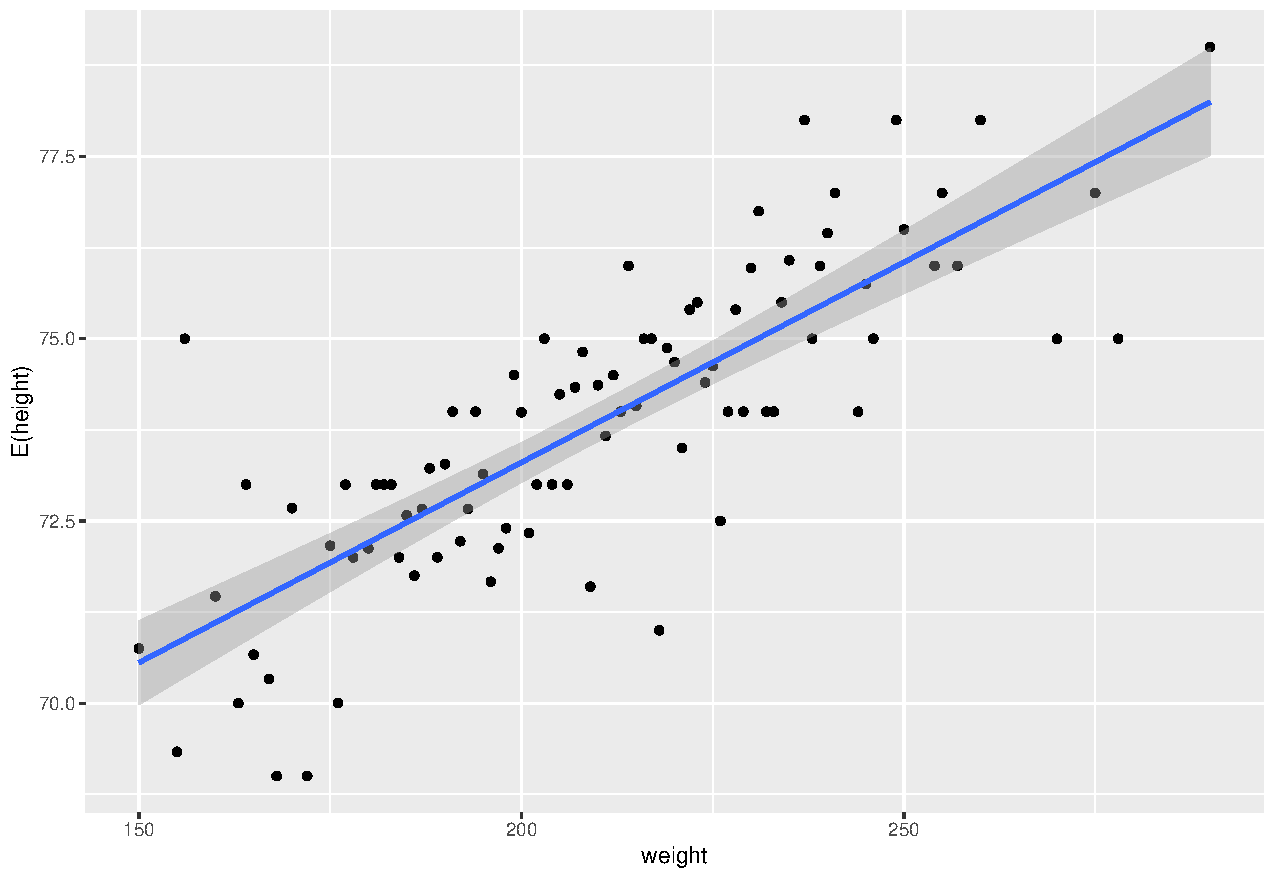
\includegraphics[width=100mm]{pictures/problemset4_scatter1.pdf}
\end{figure}
}

\frame{
\frametitle{Problem Set 4.2}
(c) Represent:
\begin{figure}
\centering
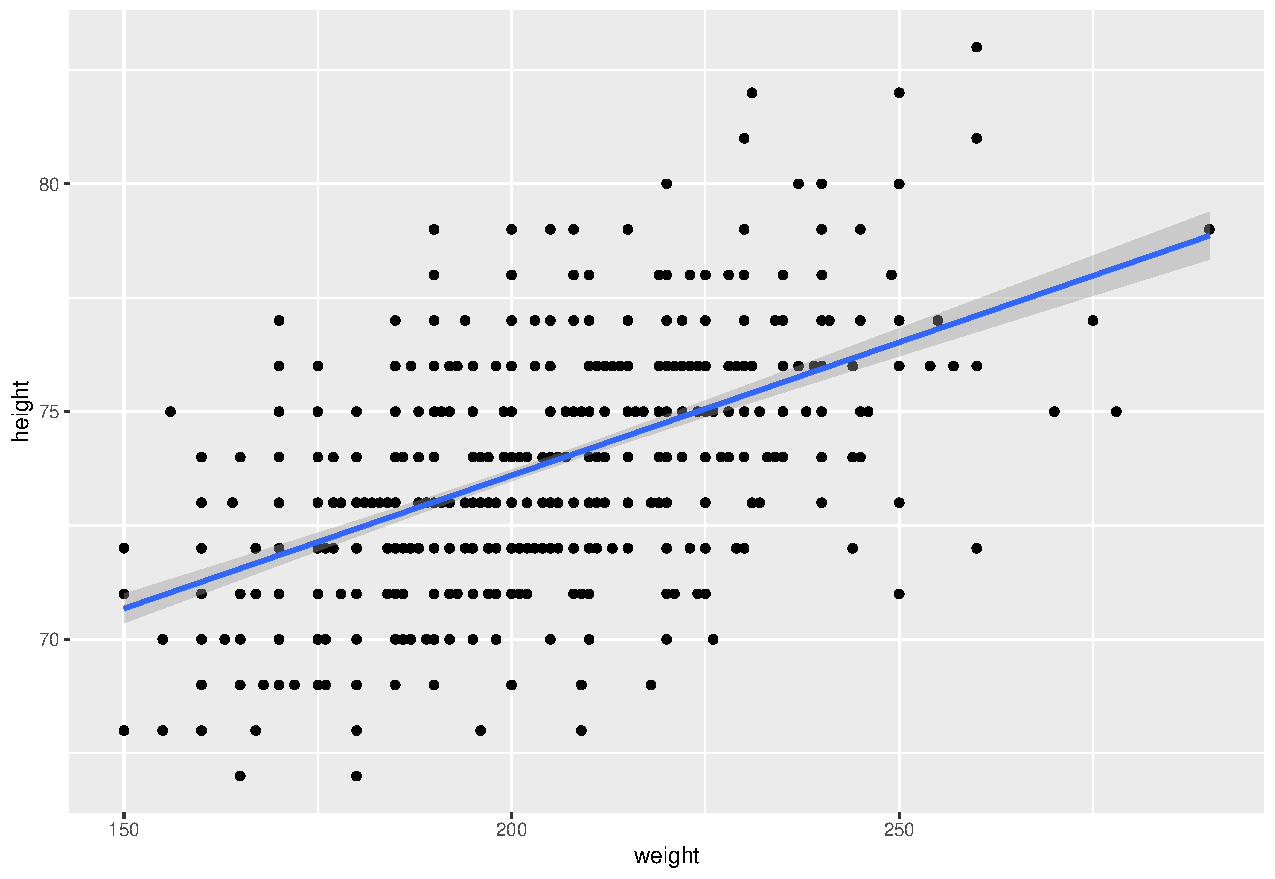
\includegraphics[width=100mm]{pictures/problemset4_scatter2.pdf}
\end{figure}
}

\begin{frame}[fragile]
\frametitle{Problem Set 4.2}
(b), (c), (d) \pause In R: 
\begin{lstlisting}[language = R]
mod1 <- lm(data = df, expected.height ~ weightpounds)
mod2 <- lm(data = data, heightinches ~ weightpounds)

stargazer(mod1, mod2,keep.stat = c("n", "adj.rsq", "f"), type = "text")
\end{lstlisting} \pause

In Stata: 
\begin{lstlisting}
egen id = group(weightpounds)
reg exp_height weightpounds if id[_n] != id[_n+1]
est store mod1

reg heightinches weightpounds
est store mod2

esttab mod1 mod2, star(* .1 ** .05 *** .01) ar2 scalars(F p) se
\end{lstlisting} 
\end{frame}

\begin{frame}
\frametitle{Problem Set 4.2}
(b), (c), (d) Results: \pause 
\begin{table}[!htbp] 
\centering 
\resizebox{80mm}{35mm}{
\begin{tabular}{@{\extracolsep{5pt}}lcc} 
\\[-1.8ex]\hline 
\hline \\[-1.8ex] 
 & \multicolumn{2}{c}{\textit{Dependent variable:}} \\ 
\cline{2-3} 
\\[-1.8ex] & E(height) & height \\ 
\\[-1.8ex] & (1) & (2)\\ 
\hline \\[-1.8ex] 
 weight & 0.055$^{***}$ & 0.058$^{***}$ \\ 
  & (0.004) & (0.003) \\ 
  & & \\ 
 Constant & 62.315$^{***}$ & 61.913$^{***}$ \\ 
  & (0.918) & (0.588) \\ 
  & & \\ 
\hline \\[-1.8ex] 
Observations & 89 & 1,033 \\ 
Adjusted R$^{2}$ & 0.645 & 0.282 \\ 
F Statistic & 161.183$^{***}$ (df = 1; 87) & 406.740$^{***}$ (df = 1; 1031) \\ 
\hline 
\hline \\[-1.8ex] 
\textit{Note:}  & \multicolumn{2}{r}{$^{*}$p$<$0.1; $^{**}$p$<$0.05; $^{***}$p$<$0.01} \\ 
\end{tabular} 
}
\end{table} 
\end{frame}

\frame{
\frametitle{Problem Set 4.2}
\begin{enumerate}
\item[(e)] (3 marks) Using the estimates of the regression of height on weight, what is the predicted height of someone who weights 225 pounds? If you do not know how to get a prediction out of your preferred statistical software, just compute by hand.
\end{enumerate} \pause
$$height=61.913 + 0.058 weight = 61.913 + 0.058 \times 225 = 74.963 $$
}

\frame{
\frametitle{Problem Set 4.2}
\begin{enumerate}
\item[(f)] 3 marks) Using the estimates of the regression of height on weight, what is the predicted height of someone who weighs 270 pounds?
\end{enumerate} \pause
$$E(height)=62.315 + 0.055 weight = 62.315 + 0.055 \times 270 = 77.165 $$
}

\frame{
\frametitle{Problem Set 4.2}
\begin{enumerate}
\item[(g)] (3 marks) Using the estimates of the regression of height on weight and if you know that So Taguchi put on 30 pounds over the winter, how much do you predict his height changed?
\end{enumerate} \pause
It's a \emph{ceteris paribus} question. Simply multiply the coefficient on weight by 30 to have the \textit{marginal} change in height. \pause He should have grown by $1.74$ inches.
}

\frame{
\frametitle{Problem Set 4.2}
\begin{enumerate}
\item[(h)] (3 marks) What do your answers to (e), (f), and (g) tell you about the interpretation of regression coefficients in general?
\end{enumerate} \pause
It gives us a correlation, the direction of the effect is up to interpretation and not just the numbers.
}

\frame{
\frametitle{Problem Set 4.3}
\begin{enumerate}
\item[3.] (24 marks) Now, let's learn how to interpret all of the regression output more thoroughly.
Input the data on campaign spending in a US Senatorial election below into your preferred statistical software:
\end{enumerate} \pause

\begin{table}
\centering
\begin{tabular}{cccc}
 District & Incumbent & Money & Vote Share\\
 1 & Matt Salmon 	& 362 	& 65 \\
 2 & Ed Pastor 		& 418 	& 68 \\
 3 & Jim Kolbe 		& 712 	& 52 \\
 4 & Bob Stump 		& 346 	& 65 \\
 5 & John Shadegg 	& 426 	& 69 \\
 6 & J.D. Hayworth 	& 1839 	& 53 \\
\end{tabular}
\end{table}
}

\frame{
\frametitle{Problem Set 4.3}
\begin{enumerate}
\item[(a)] (3 marks) Let's define the correlation between variables \textbf{M}oney and \textbf{V}ote Share as \\
\[cor(M,V) = \frac{cov(M,V)}{\sigma_M\sigma_V}\]
where the covariance of M and V is given by $cov(M,V)=1/n \sum\limits_{i=1}^{n}(m_i-\overline{m})(v_i-\overline{v})$. 
Compute $cor(M,V)$ by hand and show your computations.
Interpret the result of your computation.
Are you surprised by the result? 
Why? 
\end{enumerate}
}

\frame{
\frametitle{Problem Set 4.3}
$\overline{M}=683.83$ $\overline{V}=62$ \\ \pause
$cov(M,V)=\frac{1}{6}(((362-\overline{M})(65-\overline{V}) + (418-\overline{M})(68-\overline{V}) + (712-\overline{M})(52-\overline{V})+
  (346-\overline{M})(65-\overline{V}) + (426-\overline{M})(69-\overline{V}) + (1839-\overline{M})(53-\overline{V}))=-2676.17$ \\ \pause
$\sigma_M=581.39$ $\sigma_V=7.54$ \\ \pause
$\rho_{M,V}=\frac{-2676.17}{(581.39) (7.54)} = -0.61$ \\ \pause
There is a negative correlation between money and vote share in this senatorial election! That's interesting. Shouldn't we expect to see candidates who spend more money on their campaign get more votes? 
}

\begin{frame}[fragile]
\frametitle{Problem Set 4.3}
\begin{enumerate}
\item[(b)] (8 marks) Using your preferred statistical software, run a linear regression of V on M. \pause Plot V over M as well as the predicted values of vote share ($\hat{V}$) over M. Then add the regression line and horizontal line that indicate the residual. 
\end{enumerate} \pause In R: 
\begin{lstlisting}[language = R]
mod <- lm(data = data, vote.share ~ money)
summary(mod)
\end{lstlisting} \pause

In Stata: 
\begin{lstlisting}
reg vote_share money
\end{lstlisting} 
\end{frame}

\begin{frame}
\frametitle{Problem Set 4.3}
(b) Results: \pause
\begin{table}[!htbp] 
\centering 
\resizebox{60mm}{35mm}{
\begin{tabular}{@{\extracolsep{5pt}}lc} 
\\[-1.8ex]\hline 
\hline \\[-1.8ex] 
 & \multicolumn{1}{c}{\textit{Dependent variable:}} \\ 
\cline{2-2} 
\\[-1.8ex] & vote.share \\ 
\hline \\[-1.8ex] 
 money & $-$0.010$^{*}$ \\ 
  & (0.004) \\ 
  & \\ 
 Constant & 68.497$^{***}$ \\ 
  & (3.817) \\ 
  & \\ 
\hline \\[-1.8ex] 
Observations & 6 \\ 
Adjusted R$^{2}$ & 0.421 \\ 
F Statistic & 4.642$^{*}$ (df = 1; 4) \\ 
\hline 
\hline \\[-1.8ex] 
\textit{Note:}  & \multicolumn{1}{r}{$^{*}$p$<$0.1; $^{**}$p$<$0.05; $^{***}$p$<$0.01} \\ 
\end{tabular} 
}
\end{table} 
\end{frame}

\frame{
\frametitle{Problem Set 4.3}
(b) Plot:
\begin{figure}
\centering
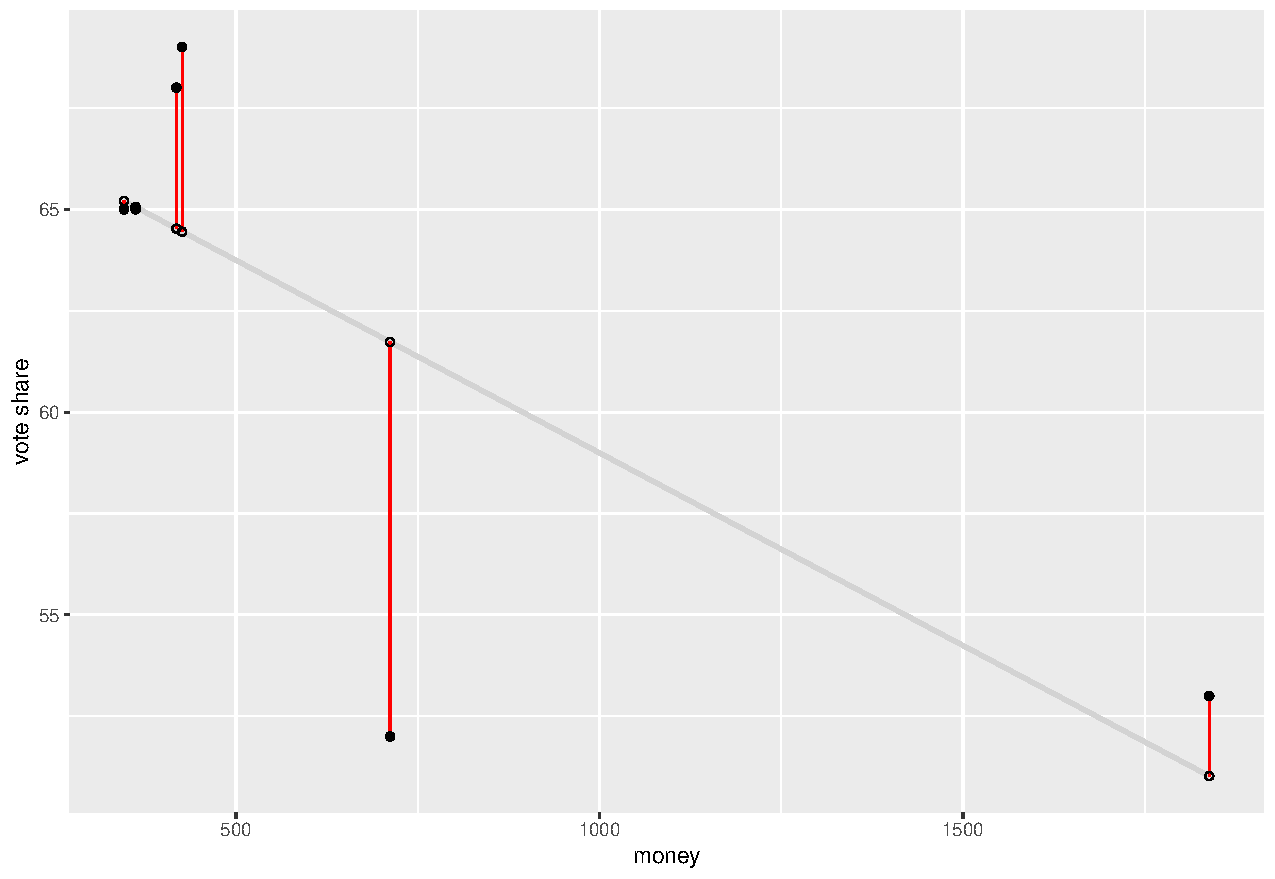
\includegraphics[width=100mm]{pictures/problemset4_scatterfit.pdf}
\end{figure}
}

\frame{
\frametitle{Problem Set 4.3}
\begin{enumerate}
\item[(b)] When you look at the coefficient estimate $\beta_M$, how is that estimate similar to the correlation between V and M you computed in 2(a)? \pause Are you surprised by the result? \pause Speculate about reasons why we see the relationship we see. \pause
\end{enumerate}

Both statistics are negative, that is, the indicate a negative relationship between M and V. \pause

You should be surprised, again, we would have expected that candidates who spend more money generate higher vote shares. \pause
 
Those candidates who won in close races (vote share closer to 50) have to spend more on their campaign because a close race means a strong challenger they had to beat (and outspend). \pause Expectations can thus reverse causality! \pause Moreover, the sample might be very selected (6 observations)
}

\frame{
\frametitle{Problem Set 4.3}
\begin{enumerate}
\item[(c)] (3 marks) Can we reject the null hypothesis that there is no relationship between V and M? 
\end{enumerate} \pause
The test distribution is the t-distribution and the t statistic in this example is $-2.155$. \pause \\
When we apply the level of significance $\alpha=.05$, we cannot reject the null hypothesis that $\beta_1 = 0$. \pause \\
The p-value is $.0975$. \pause \\
The critical values of the t-distribution for $\alpha=.05$ for a two-sided test with 4 degrees of freedom are $\pm 2.78$. \pause \\
The computed t statistic in our sample is not larger than that critical value.  
}


\frame{
\frametitle{Problem Set 4.3}
\begin{enumerate}
\item[(d)] (4 marks) Now, run a regression of V on the intercept only. 
Show your results. What does the coefficient estimate represent? \\ \pause
Generate a new variable ``m.low'' which takes on value 1 if $M<500$ and 0 otherwise. 
Run a regression of V on m.low. \pause
Compute the group-wise means of V of incumbents with low campaign spending \textit{vs} those with high campaign spending from the regression results. \pause
Show your computation.
\end{enumerate}
}

\begin{frame}[fragile]
\frametitle{Problem Set 4.3}
(d) The coefficient simply represents the mean. \pause 

In R:
\begin{lstlisting}[language = R]
mod2 <- lm(data = data, vote.share ~ vote.share)
summary(mod2)
mean(data$vote.share)
\end{lstlisting} \pause

In Stata:
\begin{lstlisting}
reg vote_share
sum vote_share
\end{lstlisting}
\end{frame}


\begin{frame}[fragile]
\frametitle{Problem Set 4.3}
(d) Ordinal variable. \pause 

In R:
\begin{lstlisting}[language = R]
# ordinal variable
data$m.low <- ifelse(data$money < 500, 1, 0)

# model
mod3 <- lm(data = data, vote.share ~ m.low)
summary(mod3)

# group-wise mean
aggregate(data$vote.share, by = list(data$m.low), FUN = mean)
\end{lstlisting}
\end{frame}

\begin{frame}[fragile]
\frametitle{Problem Set 4.3}
(d) Ordinal variable. \pause 

In Stata:
\begin{lstlisting}
* ordinal variable
gen m_low = 1 * (money < 500)

* model
reg vote_share m_low

* group-wise mean
tabstat vote_share, by(m_low)
\end{lstlisting}
\end{frame}

\frame{
\frametitle{Problem Set 4.3}
\begin{enumerate}
\item[(e)] (6 marks) Compute, by hand, the sum of squared residuals (SSR), the explained sum of squares (ESS), the total sum of squares (TSS), and $R^2$ for the regression of V on M. \pause Explain what $R^2$ tells you about model fit for this particular regression.
\end{enumerate} \pause 

$TSS=\sum\limits_{i=1}^n(y_i-\overline{y})^2$ \pause $ESS=\sum\limits_{i=1}^n(\hat{y}_i-\overline{y})^2$ \pause and $SSR=\sum\limits_{i=1}^n\hat{u}^2$ \pause

$TSS= 284$, $ESS= 152.56$, and $SSR=131.44$. \pause
$R^2=\frac{ESS}{TSS}=\frac{152.56}{284}=.5372$ (or $1-SSR/TSS$), gives the explained variance. 
}

\frame{
\frametitle{Problem Set 4.4}
\begin{enumerate}
\item[4.] (20 marks) Review how the ordinary least squares estimator is derived
\begin{enumerate}
\item[(a)] (10 marks) Derive the ordinary least squares estimator $\beta_1$ and its sampling distribution for the population model \[y=b_0 + b_1x + e.\] Show every step of your derivation. \pause
\item[(b)] (10 marks) At which steps in your derivation did you make use of the six assumptions discussed in class (week 9 slides) and the text book? Clearly indicate where you made an assumption and explain in your own words what each assumption implies.
\end{enumerate}
\end{enumerate} \pause

On the whiteboard
}

\frame{
\frametitle{Problem Set 4.5}
\begin{enumerate}
\item[5.] (17 marks) Finally, let's see why it is hard to get a causal claim out of regression analysis:
\begin{enumerate}
\item[(a)] (5 marks) Generate a 2000 observation dataset. \pause
Generate a variable ``university'' that equals 0 for the first 1000 observations and 1 for the second 1000 observations. 
This will represent half of the sample attending university. \pause
Generate a variable ``income'' which represents peoples' incomes. 
Let income = 15,000 + 5,000*university + 1,000*noise where ``noise'' is distributed standard normal. \pause

Regress income on university and show the regression output. 
\end{enumerate}
\end{enumerate}
}

\begin{frame}[fragile]
\frametitle{Problem Set 4.5}
Obtaining variables and model \\ \pause
In R: 
\begin{lstlisting}[language = R]
df <- data.frame(
  university = c(rep(0, 1000), rep(1, 1000)),
  noise = rnorm(2000)
)

df$income <- 15000 + 5000*df$university + 
             1000*df$noise

mod <- lm(data = df, income ~ university)
summary(mod)
\end{lstlisting}
\end{frame}

\begin{frame}[fragile]
\frametitle{Problem Set 4.5}
Obtaining variables and model \\ \pause
In Stata:
\begin{lstlisting}
clear
set obs 2000

gen university = 0 if _n <= 1000
replace university = 1 if _n > 1000

gen noise = rnormal()
gen income = 15000 + 5000 * university + 1000 * noise

reg income university
\end{lstlisting}
\end{frame}

\frame{
\frametitle{Problem Set 4.5}
Results:
\begin{table}[!htbp] 
\centering 
\resizebox{60mm}{35mm}{
\begin{tabular}{@{\extracolsep{5pt}}lc} 
\\[-1.8ex]\hline 
\hline \\[-1.8ex] 
 & \multicolumn{1}{c}{\textit{Dependent variable:}} \\ 
\cline{2-2} 
\\[-1.8ex] & income \\ 
\hline \\[-1.8ex] 
 university & 4,979.440$^{***}$ \\ 
  & (44.989) \\ 
  & \\ 
 Constant & 15,013.000$^{***}$ \\ 
  & (31.812) \\ 
  & \\ 
\hline \\[-1.8ex] 
Observations & 2,000 \\ 
Adjusted R$^{2}$ & 0.860 \\ 
F Statistic & 12,250.400$^{***}$ (df = 1; 1998) \\ 
\hline 
\hline \\[-1.8ex] 
\textit{Note:}  & \multicolumn{1}{r}{$^{*}$p$<$0.1; $^{**}$p$<$0.05; $^{***}$p$<$0.01} \\ 
\end{tabular} 
}
\end{table} 
}

\frame{
\frametitle{Problem Set 4.5}
\begin{enumerate}
\item[(a)] What is the coefficient estimate on university? \pause
Why should you have known before you even ran the regression what the coefficient estimate approximately will be? \pause
Is this a causal effect?
\end{enumerate} \pause

The effect of +1 university on income is $+5000$ because is what we start from in defining income itself. It is a causal effect because the 0-conditional mean assumption is met. 
}

\frame{
\frametitle{Problem Set 4.5}
\begin{enumerate}
\item[(b)] (5 marks) We now further assume that education has \textbf{no} effect on earnings, but that smart people tend to both go to university and earn more money. \pause

Clear your dataset and generate a new 2000 observation dataset. 
Generate 2 variables with uniform distributions between 0 and 1, called ``intelligence'' and ``luck.'' 
Generate a variable ``university'' which equals 1 if intelligence+luck$>$1 and 0 otherwise. \pause

Let income = 15,000 + 10,000*Intelligence + 1,000*noise where ``noise'' is distributed standard normal. \pause

Regress income on university. 
Show your the regression output.
What's your coefficient estimate on university?\\ 
\end{enumerate}
}

\begin{frame}[fragile]
\frametitle{Problem Set 4.5}
Obtaining variables and model \\ \pause
In R: 
\begin{lstlisting}[language = R]
df <- data.frame(
  intelligence = runif(2000),
  luck = runif(2000),
  noise = rnorm(2000)
)

df$university <- ifelse(df$intelligence+df$luck>1, 1, 0)
df$income <- 15000 + 10000*df$intelligence + 1000*df$noise

mod <- lm(data = df, income ~ university)
summary(mod)
\end{lstlisting}
\end{frame}

\begin{frame}[fragile]
\frametitle{Problem Set 4.5}
Obtaining variables and model \\ \pause
In Stata:
\begin{lstlisting}
clear
set obs 2000

gen intelligence = runiform()
gen luck = runiform()
gen noise = rnormal()

gen university = 1 * (intelligence + luck > 1)

gen income = 15000 + 10000 * intelligence + 1000 * noise

reg income university
\end{lstlisting}
\end{frame}

\frame{
\frametitle{Problem Set 4.5}
Results:
\begin{table}[!htbp] 
\centering 
\resizebox{60mm}{35mm}{
\begin{tabular}{@{\extracolsep{5pt}}lc} 
\\[-1.8ex]\hline 
\hline \\[-1.8ex] 
 & \multicolumn{1}{c}{\textit{Dependent variable:}} \\ 
\cline{2-2} 
\\[-1.8ex] & income \\ 
\hline \\[-1.8ex] 
 university & 3,391.231$^{***}$ \\ 
  & (117.015) \\ 
  & \\ 
 Constant & 18,331.420$^{***}$ \\ 
  & (82.990) \\ 
  & \\ 
\hline \\[-1.8ex] 
Observations & 2,000 \\ 
Adjusted R$^{2}$ & 0.296 \\ 
F Statistic & 839.902$^{***}$ (df = 1; 1998) \\ 
\hline 
\hline \\[-1.8ex] 
\textit{Note:}  & \multicolumn{1}{r}{$^{*}$p$<$0.1; $^{**}$p$<$0.05; $^{***}$p$<$0.01} \\ 
\end{tabular} 
}
\end{table} 
}


\frame{
\frametitle{Problem Set 4.5}
\begin{enumerate}
\item[(c)] (7 marks) Are the two regressions above different conceptually (that is with respect to how the regression enables us to learn something about the world)? 
Are the two regressions above different mechanically (that is with respect to how we try to get at an unbiased estimate of the true effect of university on income)?  
\end{enumerate}
}

\frame{
\frametitle{Problem Set 4.5}
\begin{enumerate}
\item Conceptually, the first represents clean experimental data (university is randomly assigned and normally distributed error term independent of university). \pause Causal effect of University on wage. \pause In this case, we know the DGP \pause
\item The second has university confounded by intelligence and luck. \pause OVB because luck affects our estimate of the effect of university on wage through the error term. \pause In this case, we do not know the DGP \pause
\item We should have modelled wages as function of intelligence \textbf{and} luck. \pause
\item Mechanically, in the second case we are trying to estimate a coefficient on university which is a compound of the effect of intelligence and luck.
\end{enumerate}
}


\frame{
\frametitle{Conclusion}
\begin{center}
All clear? Questions? \\
Thanks and see you next week!
\end{center}
}

%\begin{frame}
%\bibliographystyle{apalike}
%\bibliography{week_10.bib}
%\end{frame}

\end{document}